\chapter{Entity Relationship Diagram (ERD)}
\label{ch:erd}

% Diagram first
\begin{figure}[H]
\centering
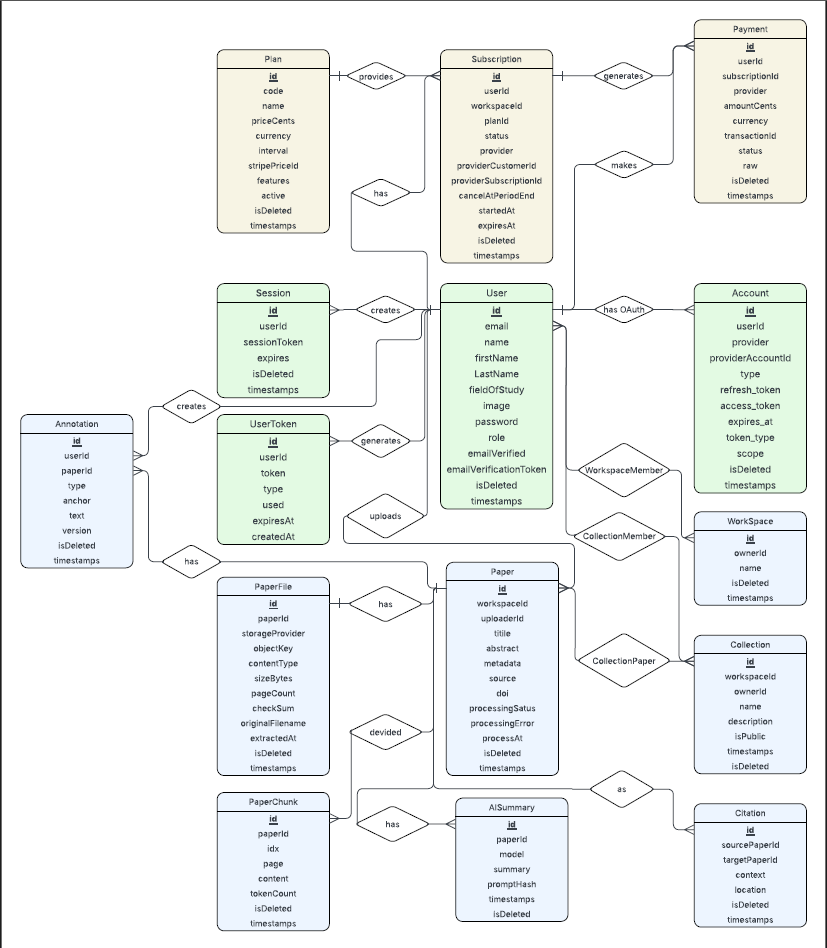
\includegraphics[width=0.95\textwidth]{images/diagrams/ERD.png}
\caption{ScholarFlow Entity Relationship Diagram}
\label{fig:erd-complete}
\end{figure}

% One-page key information
\section*{Key Information}
\begin{itemize}[leftmargin=*,topsep=3pt,itemsep=2pt]
  \item \textbf{Technology}: PostgreSQL 15+, Prisma (RAW Query) for data access, migrations via Prisma Migrate.
  \item \textbf{Domains}: Users, Papers, Collections, Workspaces, AI, Billing.
  \item \textbf{Relationships}: One-to-many (User \texorpdfstring{$\rightarrow$}{->} Paper), many-to-many (Collection \texorpdfstring{$\leftrightarrow$}{<->} Paper via join table).
  \item \textbf{Integrity}: Foreign keys enforced; unique constraints on emails and composite keys (e.g., workspaceId+userId).
  \item \textbf{Soft Delete}: isDeleted + deletedAt on key entities; queries filter active records.
  \item \textbf{Indexes}: Composite indexes on hot paths (uploaderId+workspaceId, workspaceId+isDeleted); text search on titles/abstracts when applicable.
  \item \textbf{Scalability}: Paginated reads, parameterized RAW queries, and selective denormalized counts for dashboards.
\end{itemize}
